\Exhibit{FceDemo}{%
    Скриншот Apache Beam Playground -- приложения, использующего Flutter Code Editor%
}

Этот скриншот показывает Apache Beam Playground -- приложение, которое Akvelon разработал
для \Asf.
У него много функций.
В центральной части редактор -- это `Flutter Code Editor',
продукт Akvelon, который можно использовать в разных приложениях.

На скриншоте:

\begin{itemize}
    \item Строки 2--17, 19--31 и 34--58 свёрнуты, чтобы не отвлекать программиста.
    \item Автодополнение предлагает слово по мере печати.
    \item Крестики показывают ошибки.
    \item Один из крестиков показывает текст ошибки, если навести мышь.
\end{itemize}

Уникальность Flutter Code Editor в том, что все эти функции сейчас работают в браузере,
но могут работать и в мобильном приложении на iOS и Android без усилией.

\begin{center}
    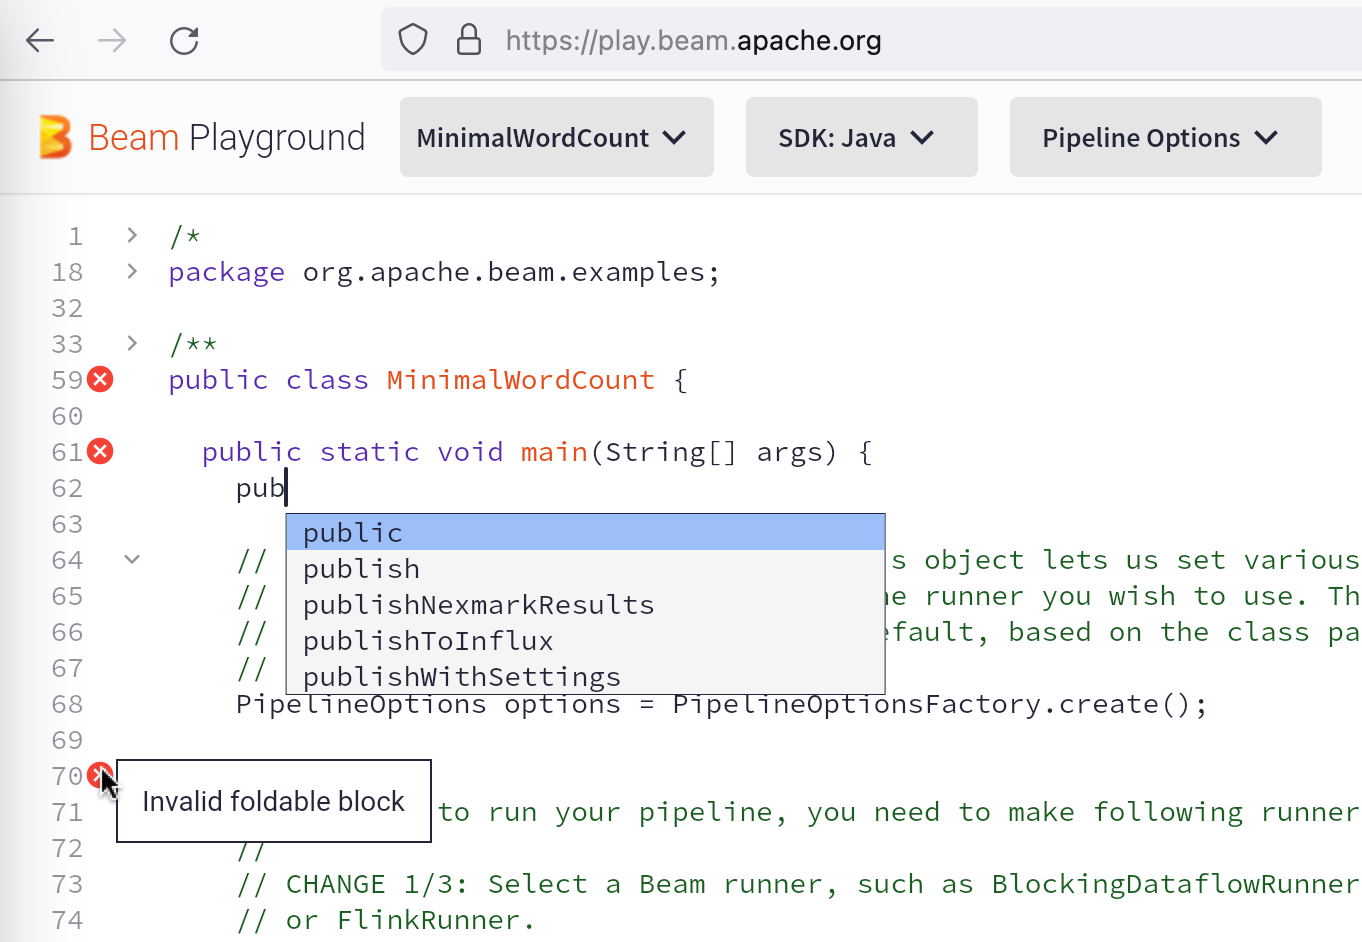
\includegraphics[width=30em]{demo}
\end{center}

\pagebreak
